Each electrical component has a specific power requirement and this layer is responsible for providing that power.

\subsection{Battery}
This module consists of a Li-Po battery which provides power to a Buck Converter.

\begin{figure}[h!]
	\centering
 	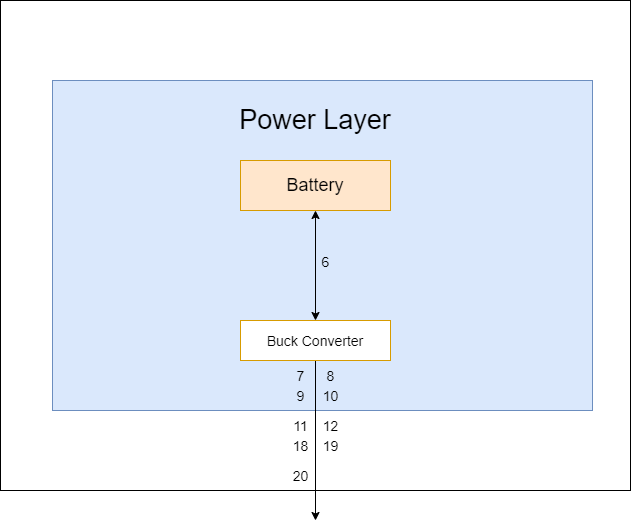
\includegraphics[width=0.60\textwidth]{images/Bat.png}
 \caption{Battery Subsystem in Power Layer}
\end{figure}

\subsubsection{Assumptions}
The batteries are expected to allow the user to ride the longboard for at least 30 minutes without requiring recharging.

\subsubsection{Responsibilities}
The Batteries would ideally provide around 24V.

\subsubsection{Subsystem Interfaces}
Each of the inputs and outputs for the subsystem are defined here.

\begin {table}[H]
\caption {Battery interfaces} 
\begin{center}
    \begin{tabular}{ | p{1cm} | p{6cm} | p{3cm} | p{3cm} |}
    \hline
    ID & Description & Inputs & Outputs \\ \hline
    \#6 & Raw Power & \pbox{3cm}{Excess power} & \pbox{3cm}{24V}  \\ \hline
    \end{tabular}
\end{center}
\end{table}

\subsection{Buck Converter}
The entire module consists of a Li-Po battery which provides power to a Buck Converter which then powers the rest of the system.

\begin{figure}[h!]
	\centering
 	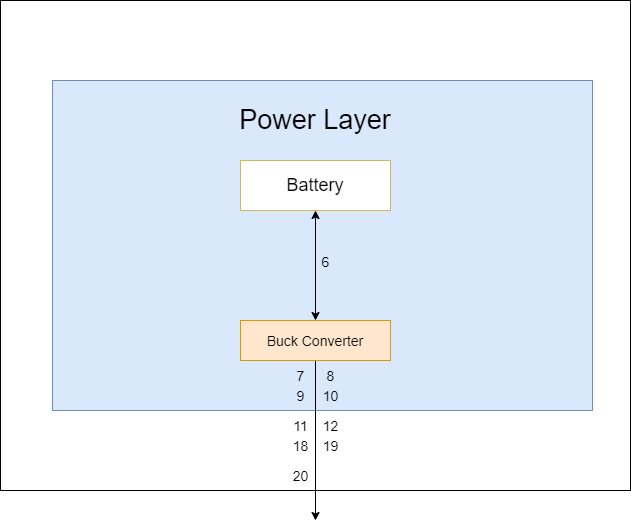
\includegraphics[width=0.60\textwidth]{images/Buck.png}
 \caption{Buck Converter Subsystem in Power Layer}
\end{figure}

\subsubsection{Assumptions}
The batteries are expected to allow the user to ride the longboard for at least 30 minutes without requiring recharging.

\subsubsection{Responsibilities}
The Buck converter will take the 24V from the battery and step it down to 19V for the Jetson TX-2 and 5V if an auxiliary micro-controller is connected.

\subsubsection{Subsystem Interfaces}
Each of the inputs and outputs for the subsystem are defined here.

\begin {table}[H]
\caption {Buck converter interfaces} 
\begin{center}
    \begin{tabular}{ | p{1cm} | p{6cm} | p{3cm} | p{3cm} |}
    \hline
    ID & Description & Inputs & Outputs \\ \hline
    \#7 & Power Delivery to Jetson & \pbox{3cm}{N/A} & \pbox{3cm}{19V/5V}  \\ \hline
    \#8 & Power Delivery to Microcontroller & \pbox{3cm}{N/A} & \pbox{3cm}{19V/5V}  \\ \hline
    \#9 & Power Delivery to ESC & \pbox{3cm}{N/A} & \pbox{3cm}{19V/5V}  \\ \hline
    \#10 & Power Delivery to Brushless DC & \pbox{3cm}{N/A} & \pbox{3cm}{19V/5V}  \\ \hline
    \#11 & Power Delivery to Solenoids & \pbox{3cm}{N/A} & \pbox{3cm}{19V/5V}  \\ \hline
    \#12 & Power Delivery to Stepper Motor & \pbox{3cm}{N/A} & \pbox{3cm}{19V/5V}  \\ \hline
    \#18 & Power Delivery to Weight Sensor & \pbox{3cm}{N/A} & \pbox{3cm}{19V/5V}  \\ \hline
    \#19 & Power Delivery to LED Strip & \pbox{3cm}{N/A} & \pbox{3cm}{19V/5V}  \\ \hline
    \#20 & Power Delivery to Buzzer/Speaker  & \pbox{3cm}{N/A} & \pbox{3cm}{19V/5V}  \\ \hline
\end{tabular}
\end{center}
\end{table}